\chapter{Simulationergebnisse}

\section{Alliance Memory}
\label{app:alliance}
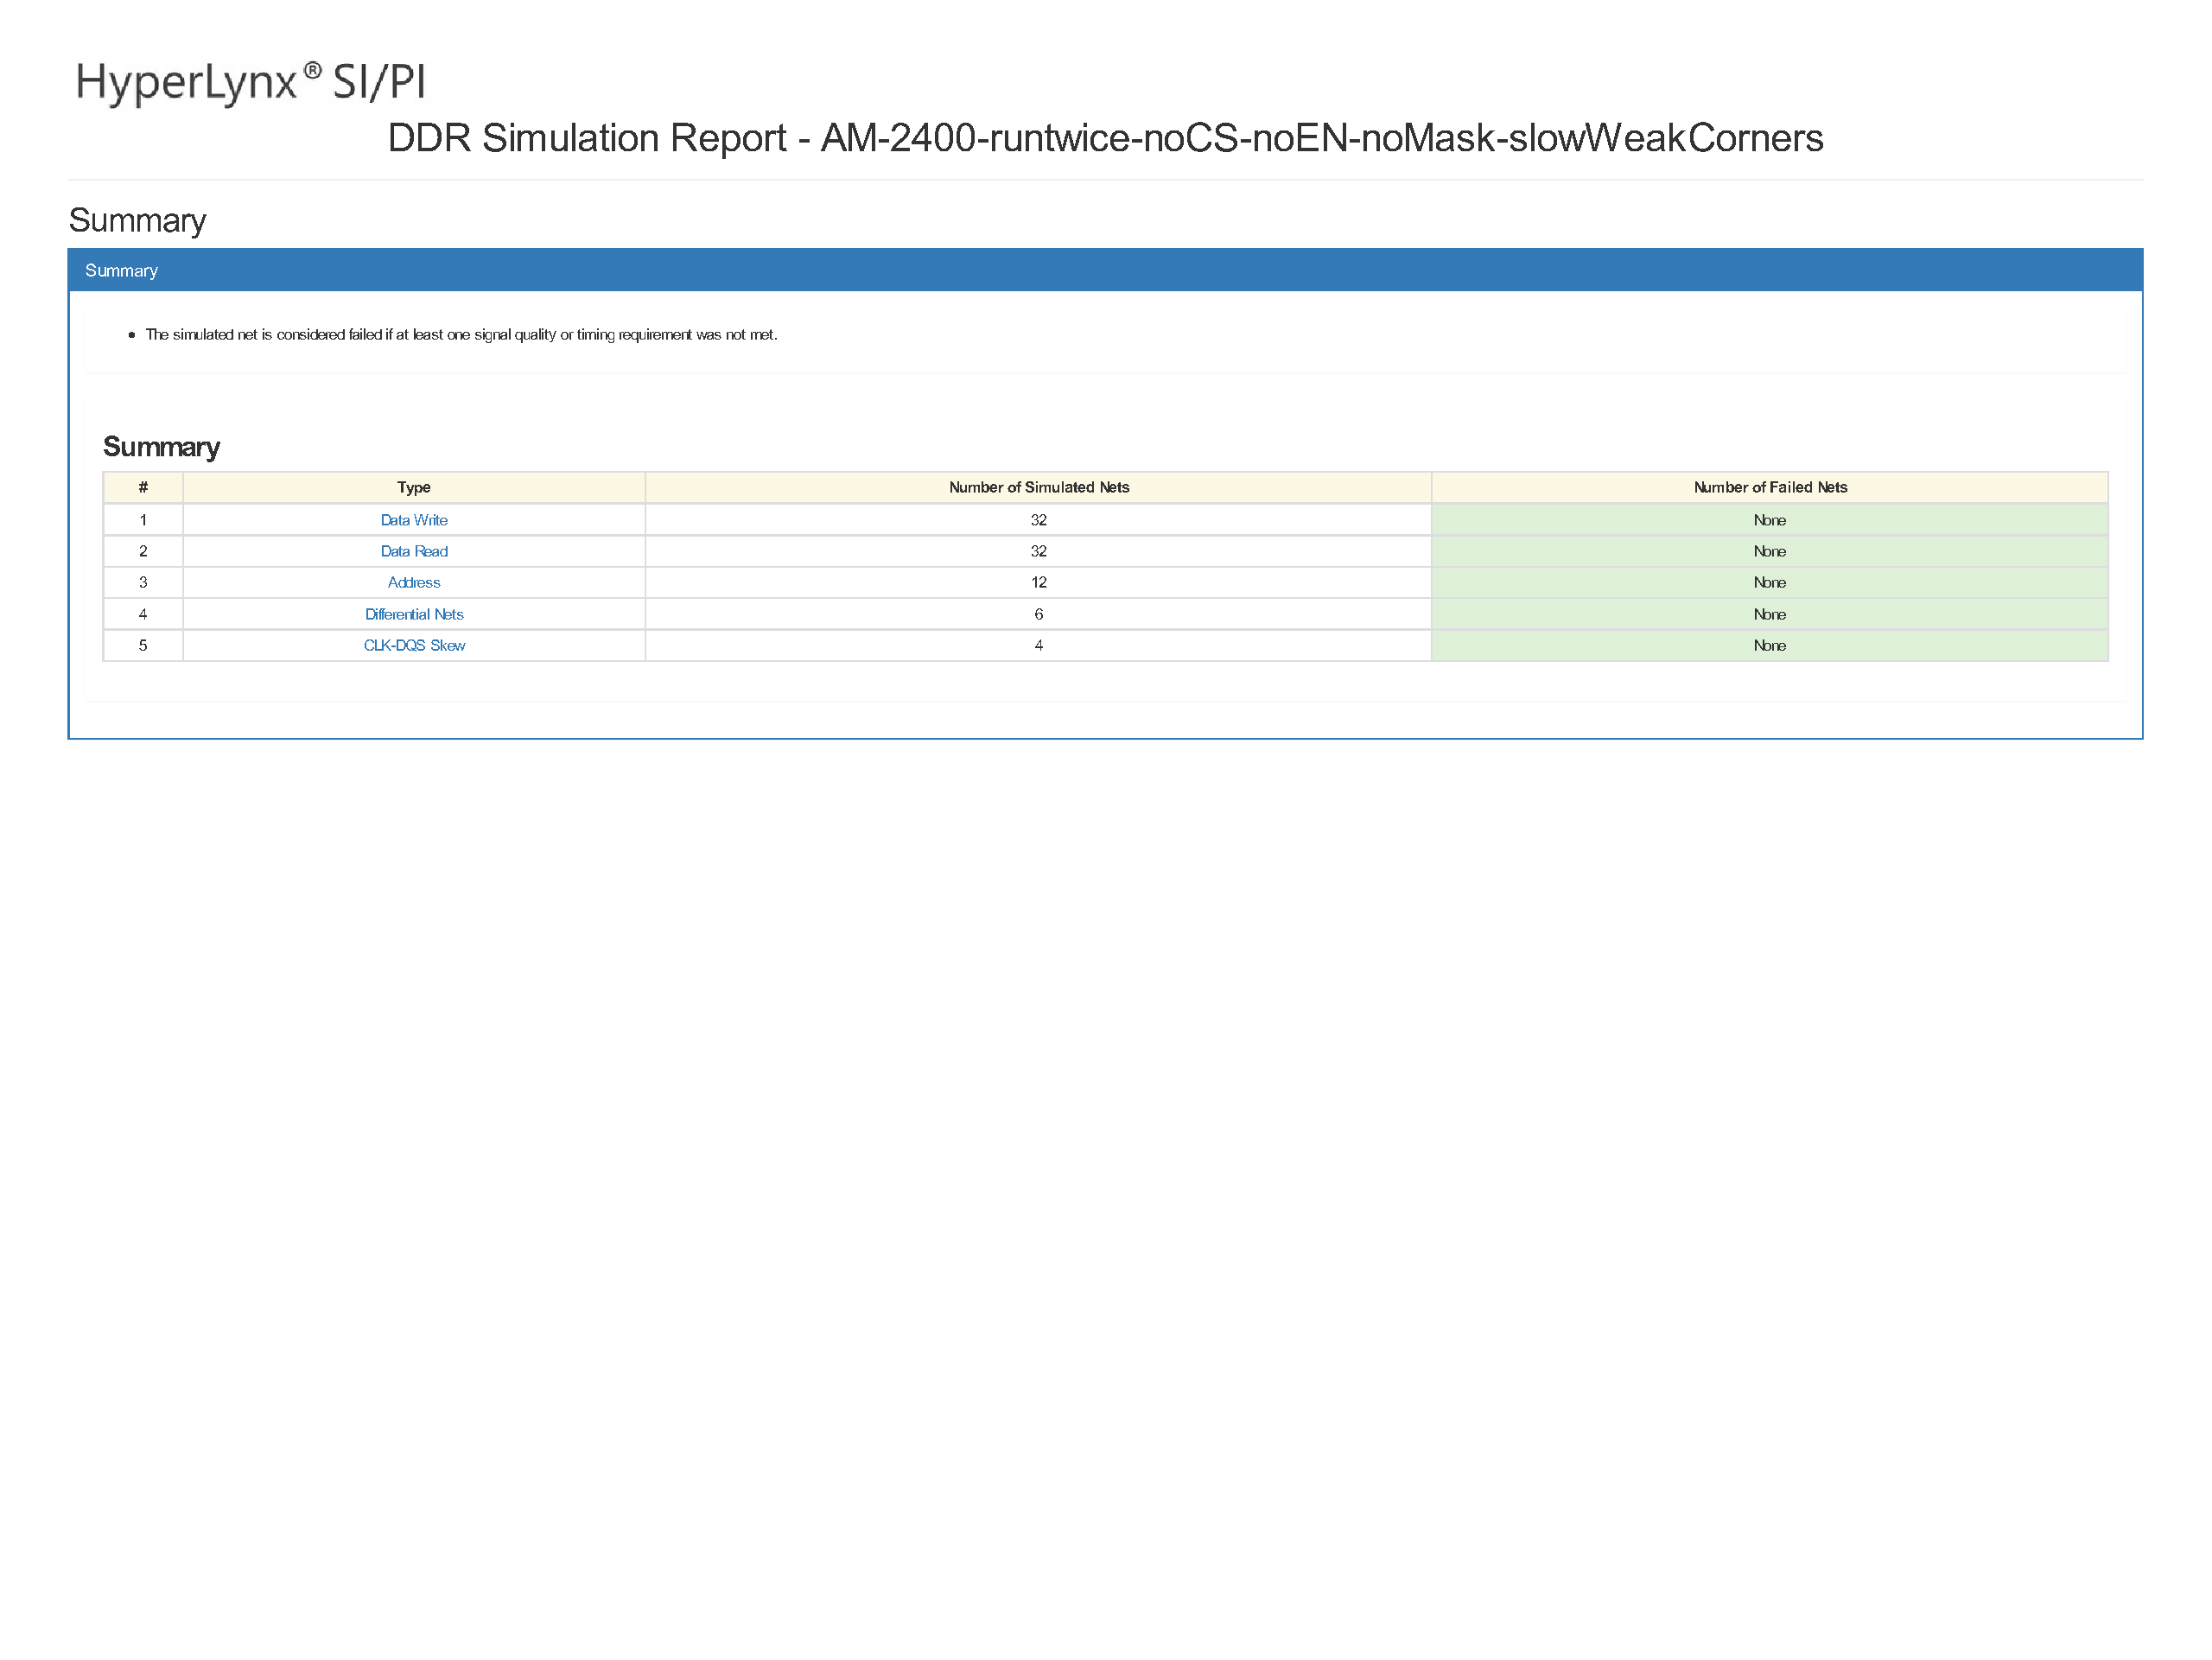
\includepdf[
    pages=-,                % Bindet alle Seiten des PDFs ein (oder z.B. pages={1-3})
    scale=0.85,             % Skaliert das PDF leicht, damit es in den Satzspiegel passt
    pagecommand={\thispagestyle{plain}}, % Behält die normale Seitenzahl bei (z.B. Unten mittig)
    angle=90,                % Falls das PDF im Querformat ist, hier z.B. 90 eintragen
    frame=true              % Optional: Zeichnet einen feinen Rahmen um die Seite
]{datasheets/AM_DDR_report.pdf}

\section{Intelligent Memory}
\label{app:intelligent}
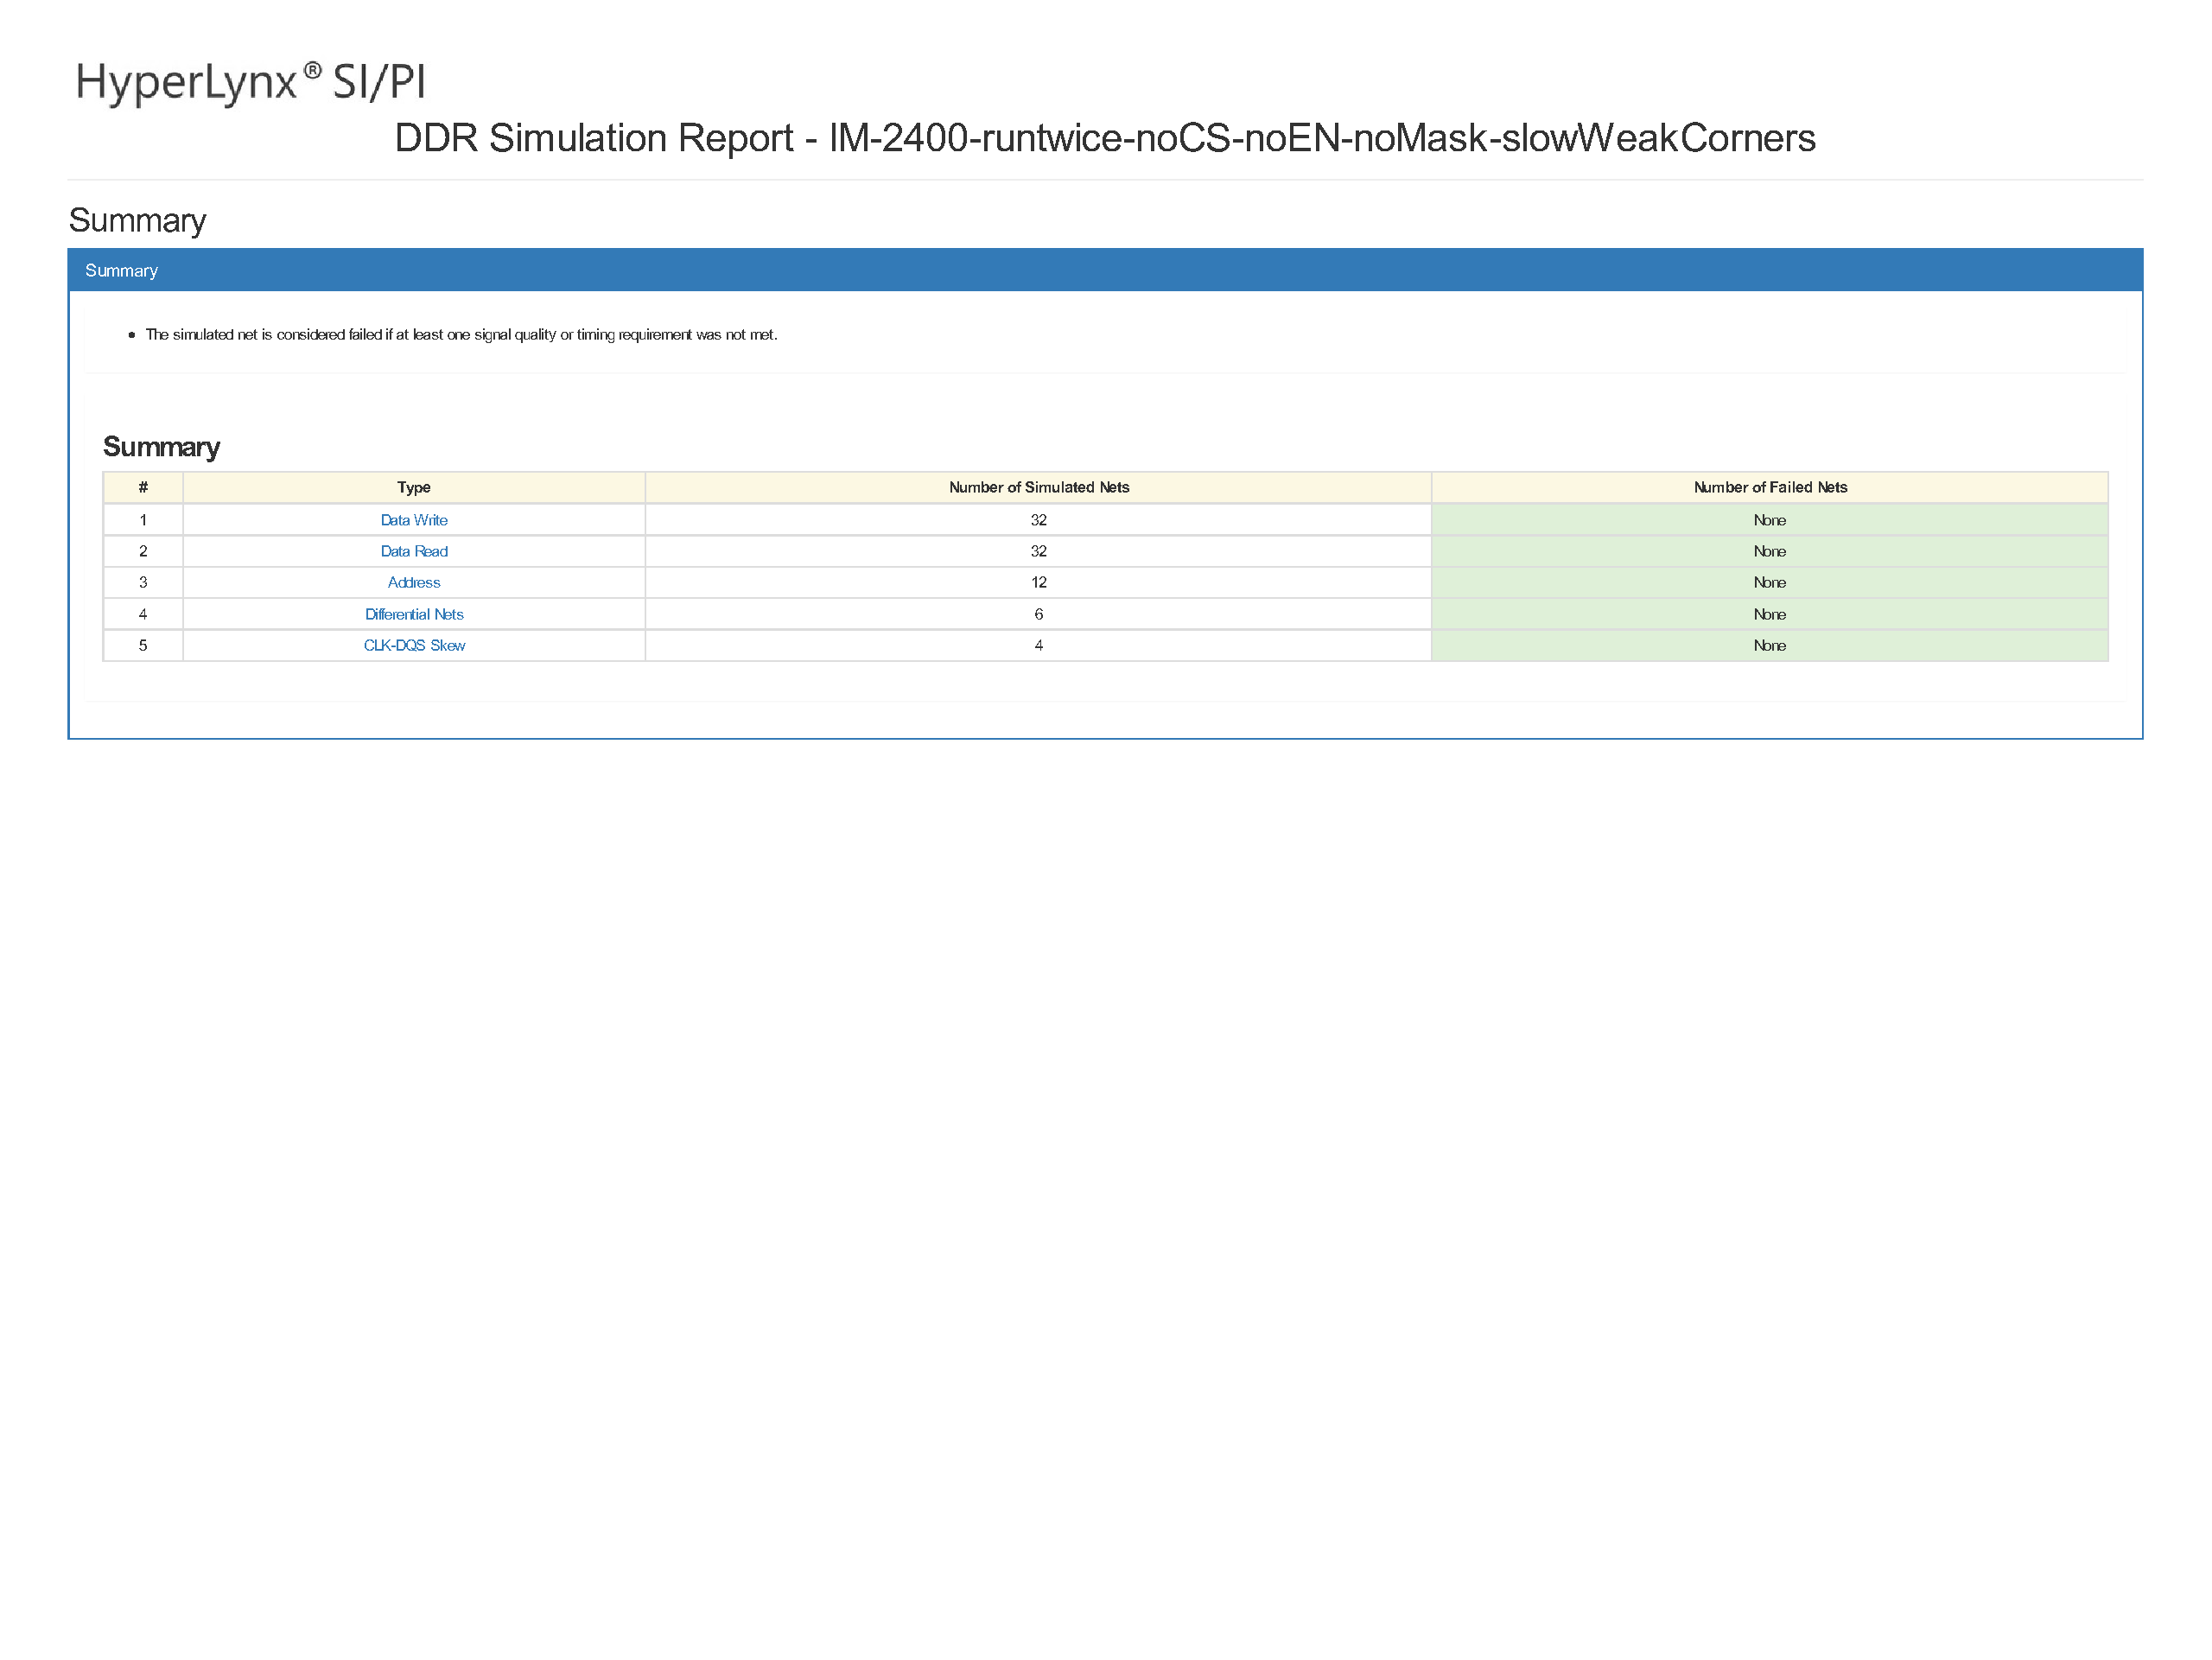
\includepdf[
    pages=-,
    scale=0.85,
    pagecommand={\thispagestyle{plain}},
    angle=90,
    frame=true
]{datasheets/IM_DDR_report.pdf}

\section{\gls{issi}}
\label{app:issi}
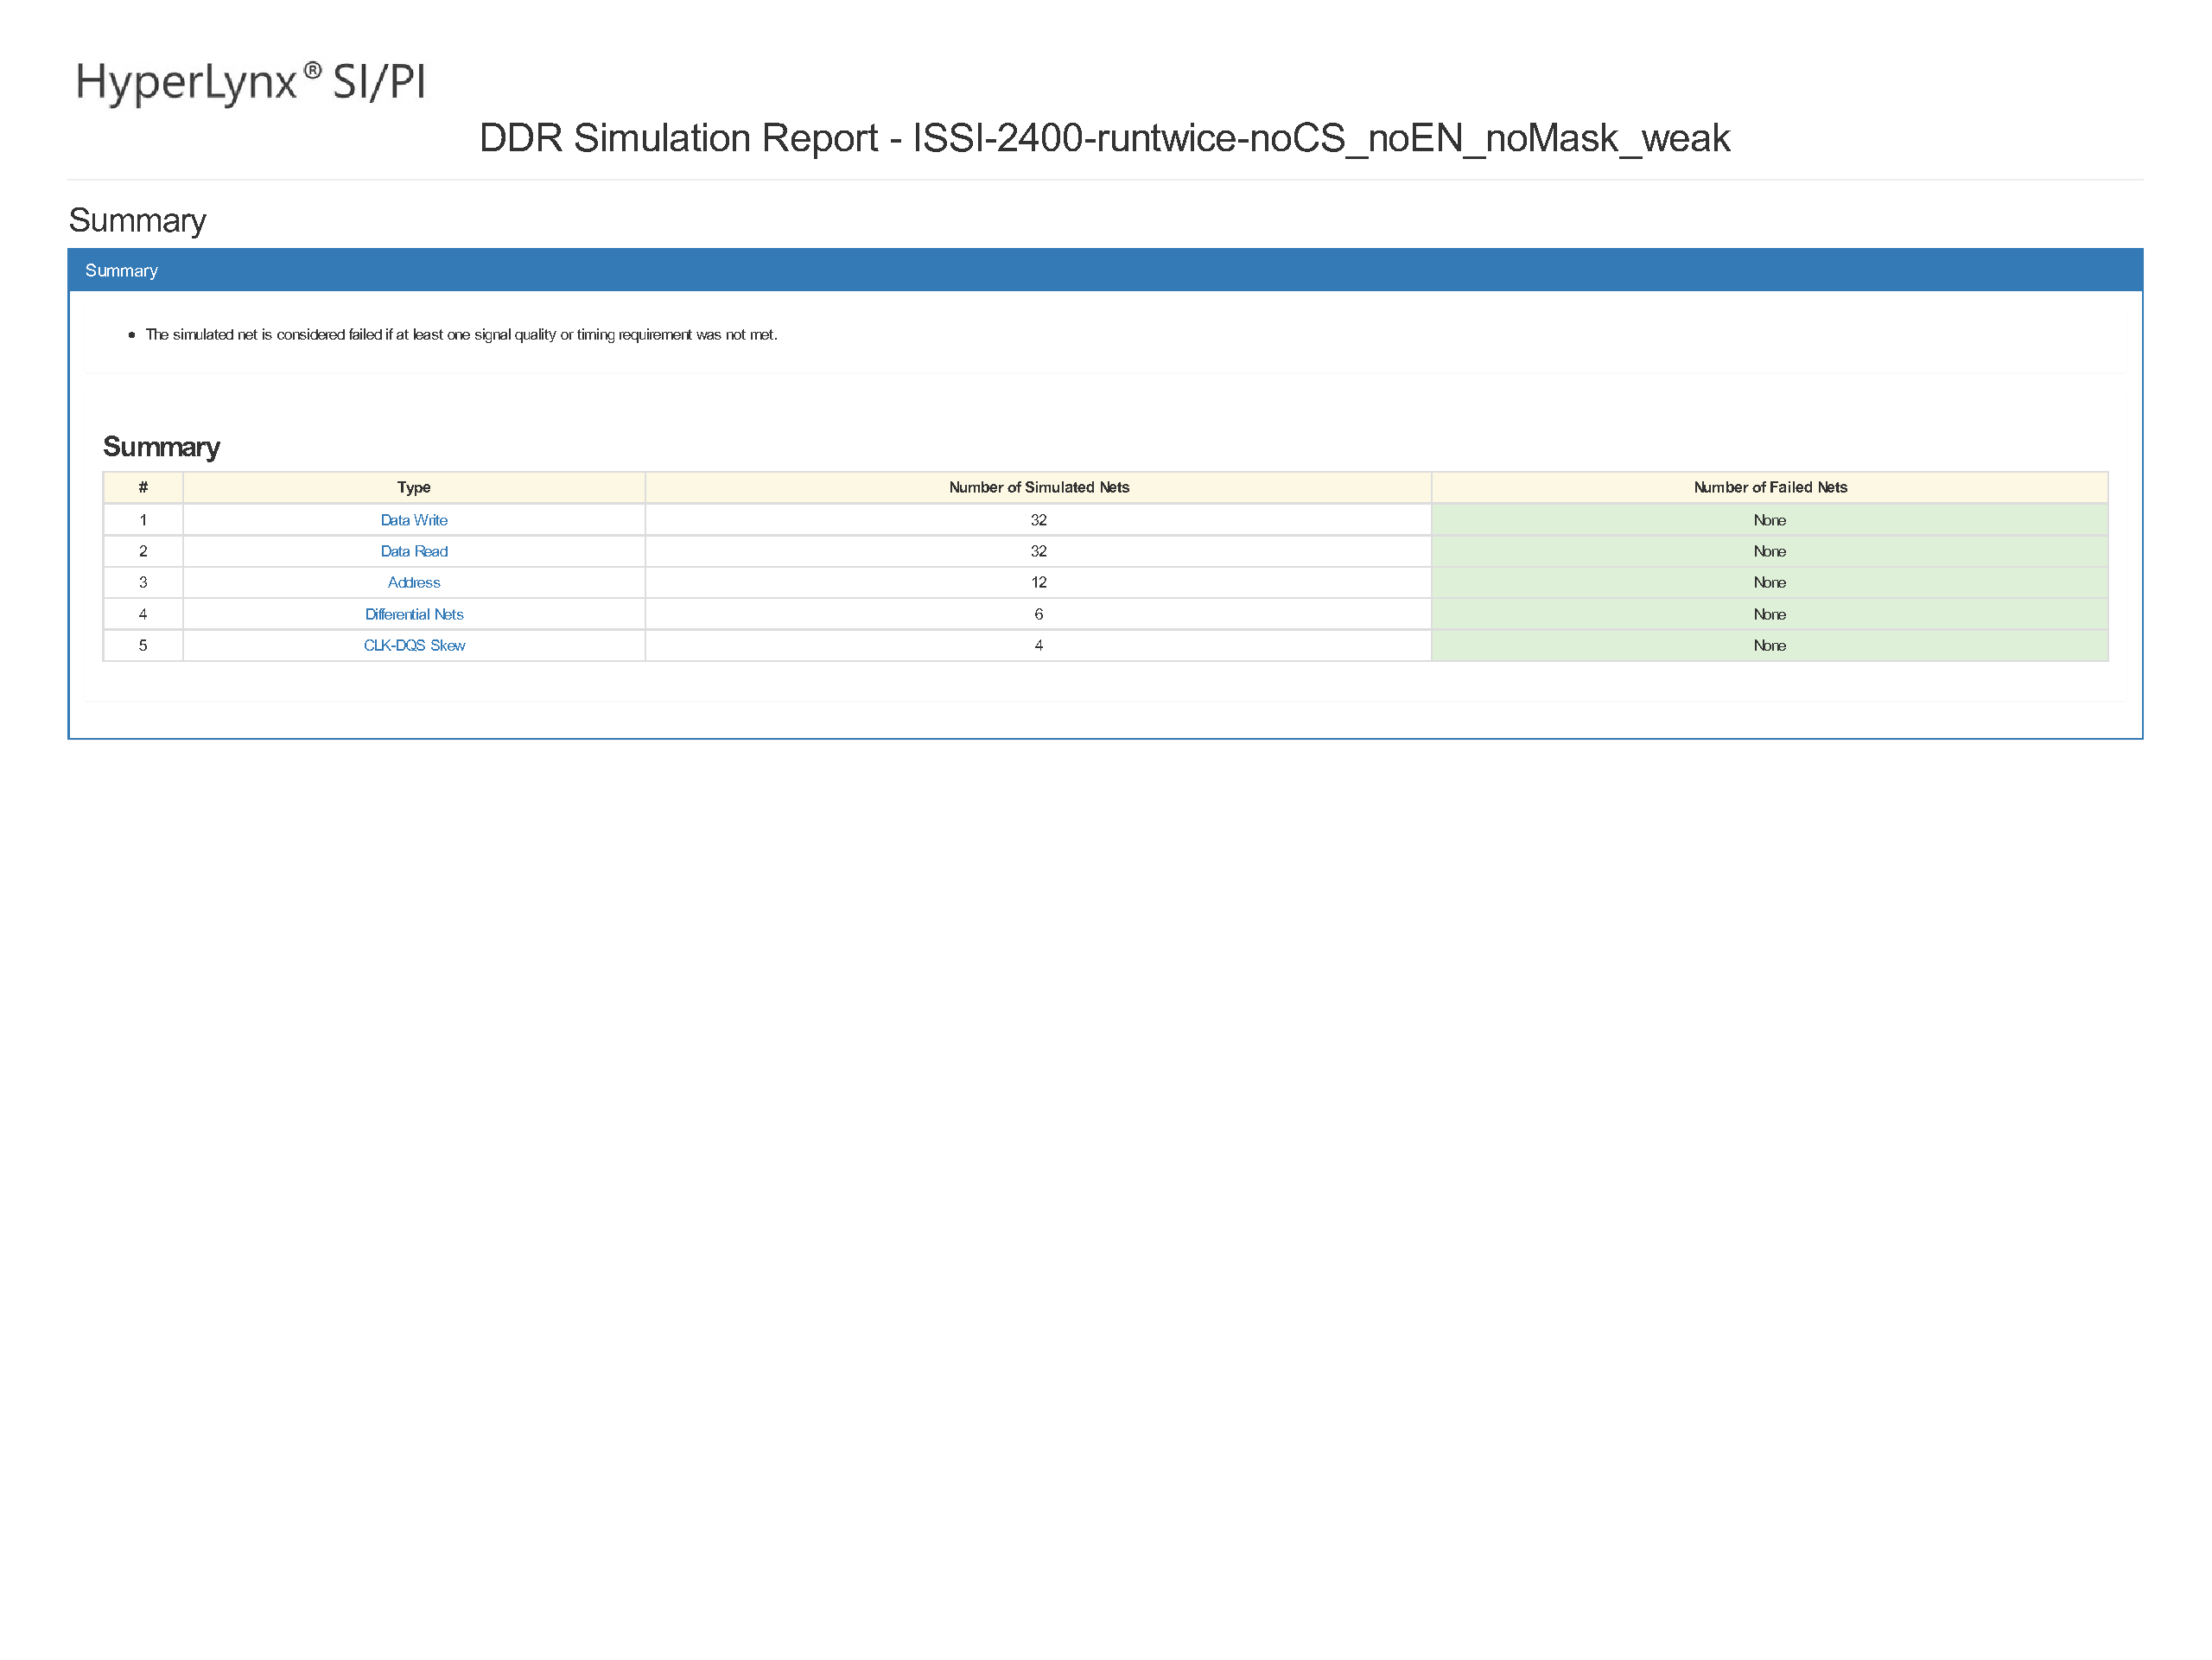
\includepdf[
    pages=-,
    scale=0.85,
    pagecommand={\thispagestyle{plain}},
    angle=90,
    frame=true
]{datasheets/ISSI_DDR_report.pdf}

\chapter{Layout}
\label{app:layout}
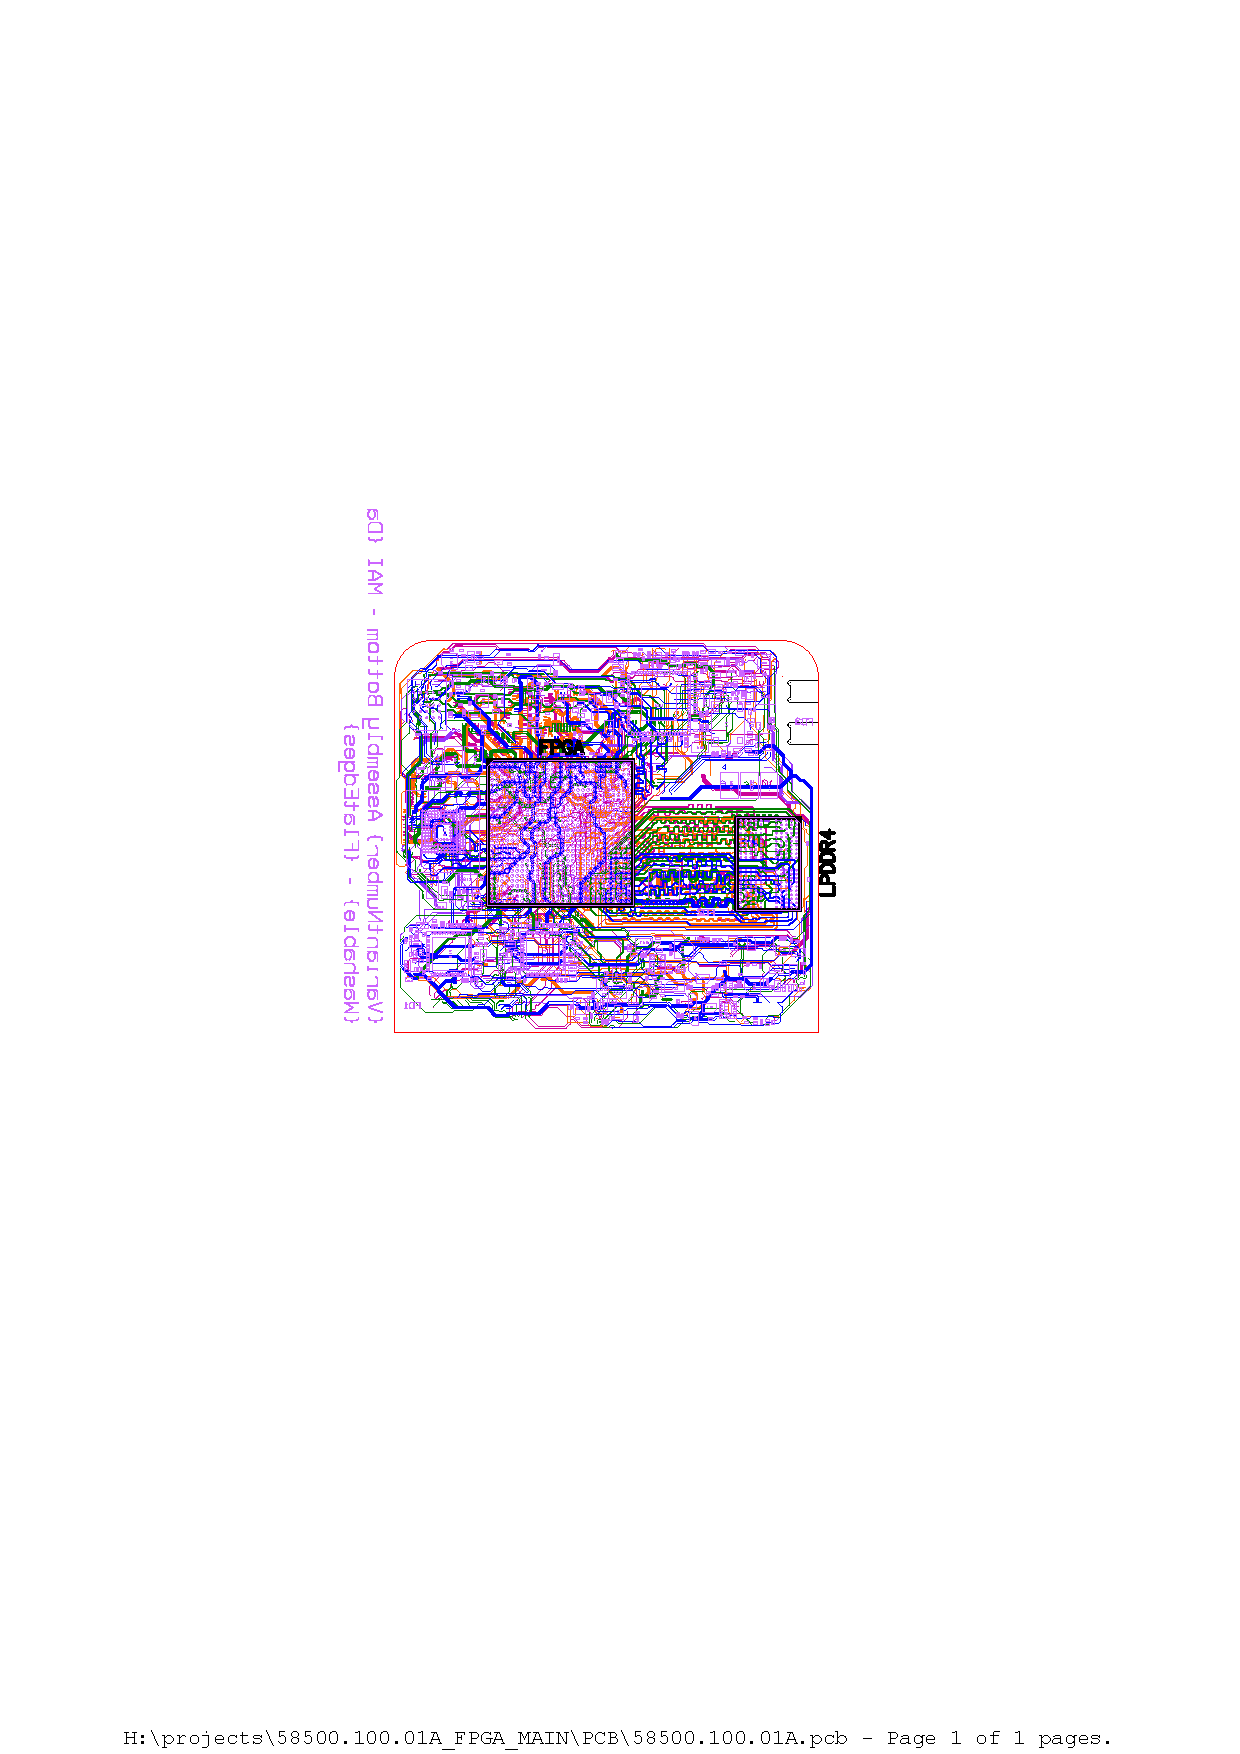
\includepdf[
    pages=-,
    scale=0.85,
    pagecommand={\thispagestyle{plain}},
    angle=00,
    frame=true
]{datasheets/routing-fpga-lpddr4.pdf}